97. а) $f(x)=\begin{cases} \cfrac{3x+1}{x-1},\ x\neq1\\3+1,\ x=1 \end{cases}=\begin{cases} 3+\cfrac{4}{x-1},\ x\neq1\\ 4,\ x=1 \end{cases}.$
$$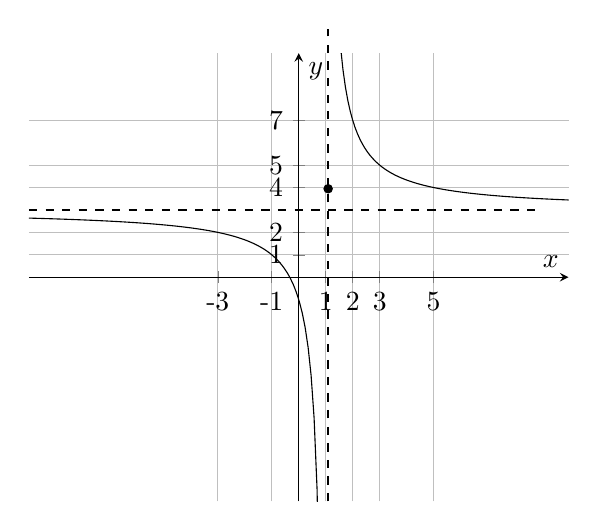
\begin{tikzpicture}[scale=1]
\tikzset{line03/.style={dashed,line width =0.9pt}}
\begin{axis}[
    axis lines = middle,
    grid=major,
    legend pos={south west},
    xlabel = {$x$},
    %xlabel style={below right},
    ylabel = {$y$},
    ymin=-10,
    ymax=10,
    xmin=-10,
    xmax=10,
    xtick={ -3, -1, 1, 2, 3, 5},
    xticklabels={ -3, -1, $\text{1     }$, 2, 3, 5},
    ytick={2, 1, 7, 5, 4},
    yticklabels={$\text{2}$,$\text{1}$, $\text{7}$, $\text{5}$, $\text{4}$},        ]

	\addplot[domain=1.1:10, samples=100, color=black] {3+4/(x-1)};
	\addplot[domain=-10:0.9, samples=100, color=black] {3+4/(x-1)};

\end{axis}
\filldraw [black] (3.8,3.97) circle (1.5pt);
\draw[line03] (3.8,0) -- (3.8,6);
\draw[line03] (0,3.7) -- (6.5,3.7);
%\draw (3,5.7) node {\scriptsize $y$};
%\draw (7,2.5) node {\scriptsize $x$};
\end{tikzpicture}$$
б) Горизонтальная прямая $y=a+1$ не пересекается с графиком данной функции только в том случае, если является его асимптотой, то есть $a+1=3,\ a=2.$\\
в) Прямая $y=ax+2$ имеет с графиком три общие точки, только если она пересекает гиперболу 2 раза (тогда $a>0$) и проходит через изолированную точку $(1;3-a).$ Тогда $a+2=3-a,\ 2a=1,\ a=\cfrac{1}{2}.$\\
